\section*{Experiment 1}

\begin{figure}[H]
\centering
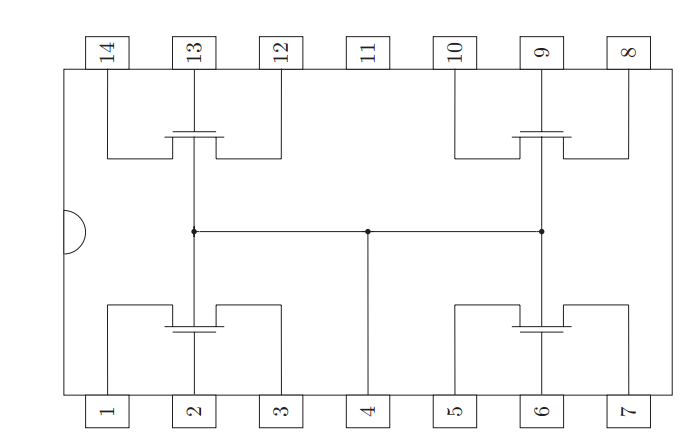
\includegraphics[width=0.65\linewidth]{../Figures/ald1106}
\caption{Picture of the ALD1106 QUAD nMOS transistor array which was used in Experiment 1 to analyze the similarities between nMOS transistors. Using a Quad array is ideal as all transistors are manufactured on the same substrate, optimizing their similarity.}
\label{fig:ald1106}
\end{figure}


In this experiment, we wanted to evaluate how well-matched four nMOS transistors on the same die are. We used the ALD1106 Quad nMOS array, as seen in figure \ref{fig:ald1106}, as all four transistors on this chip are manufactured on the same substrate, which optimizes their similarity.

\begin{figure}[H]
\centering
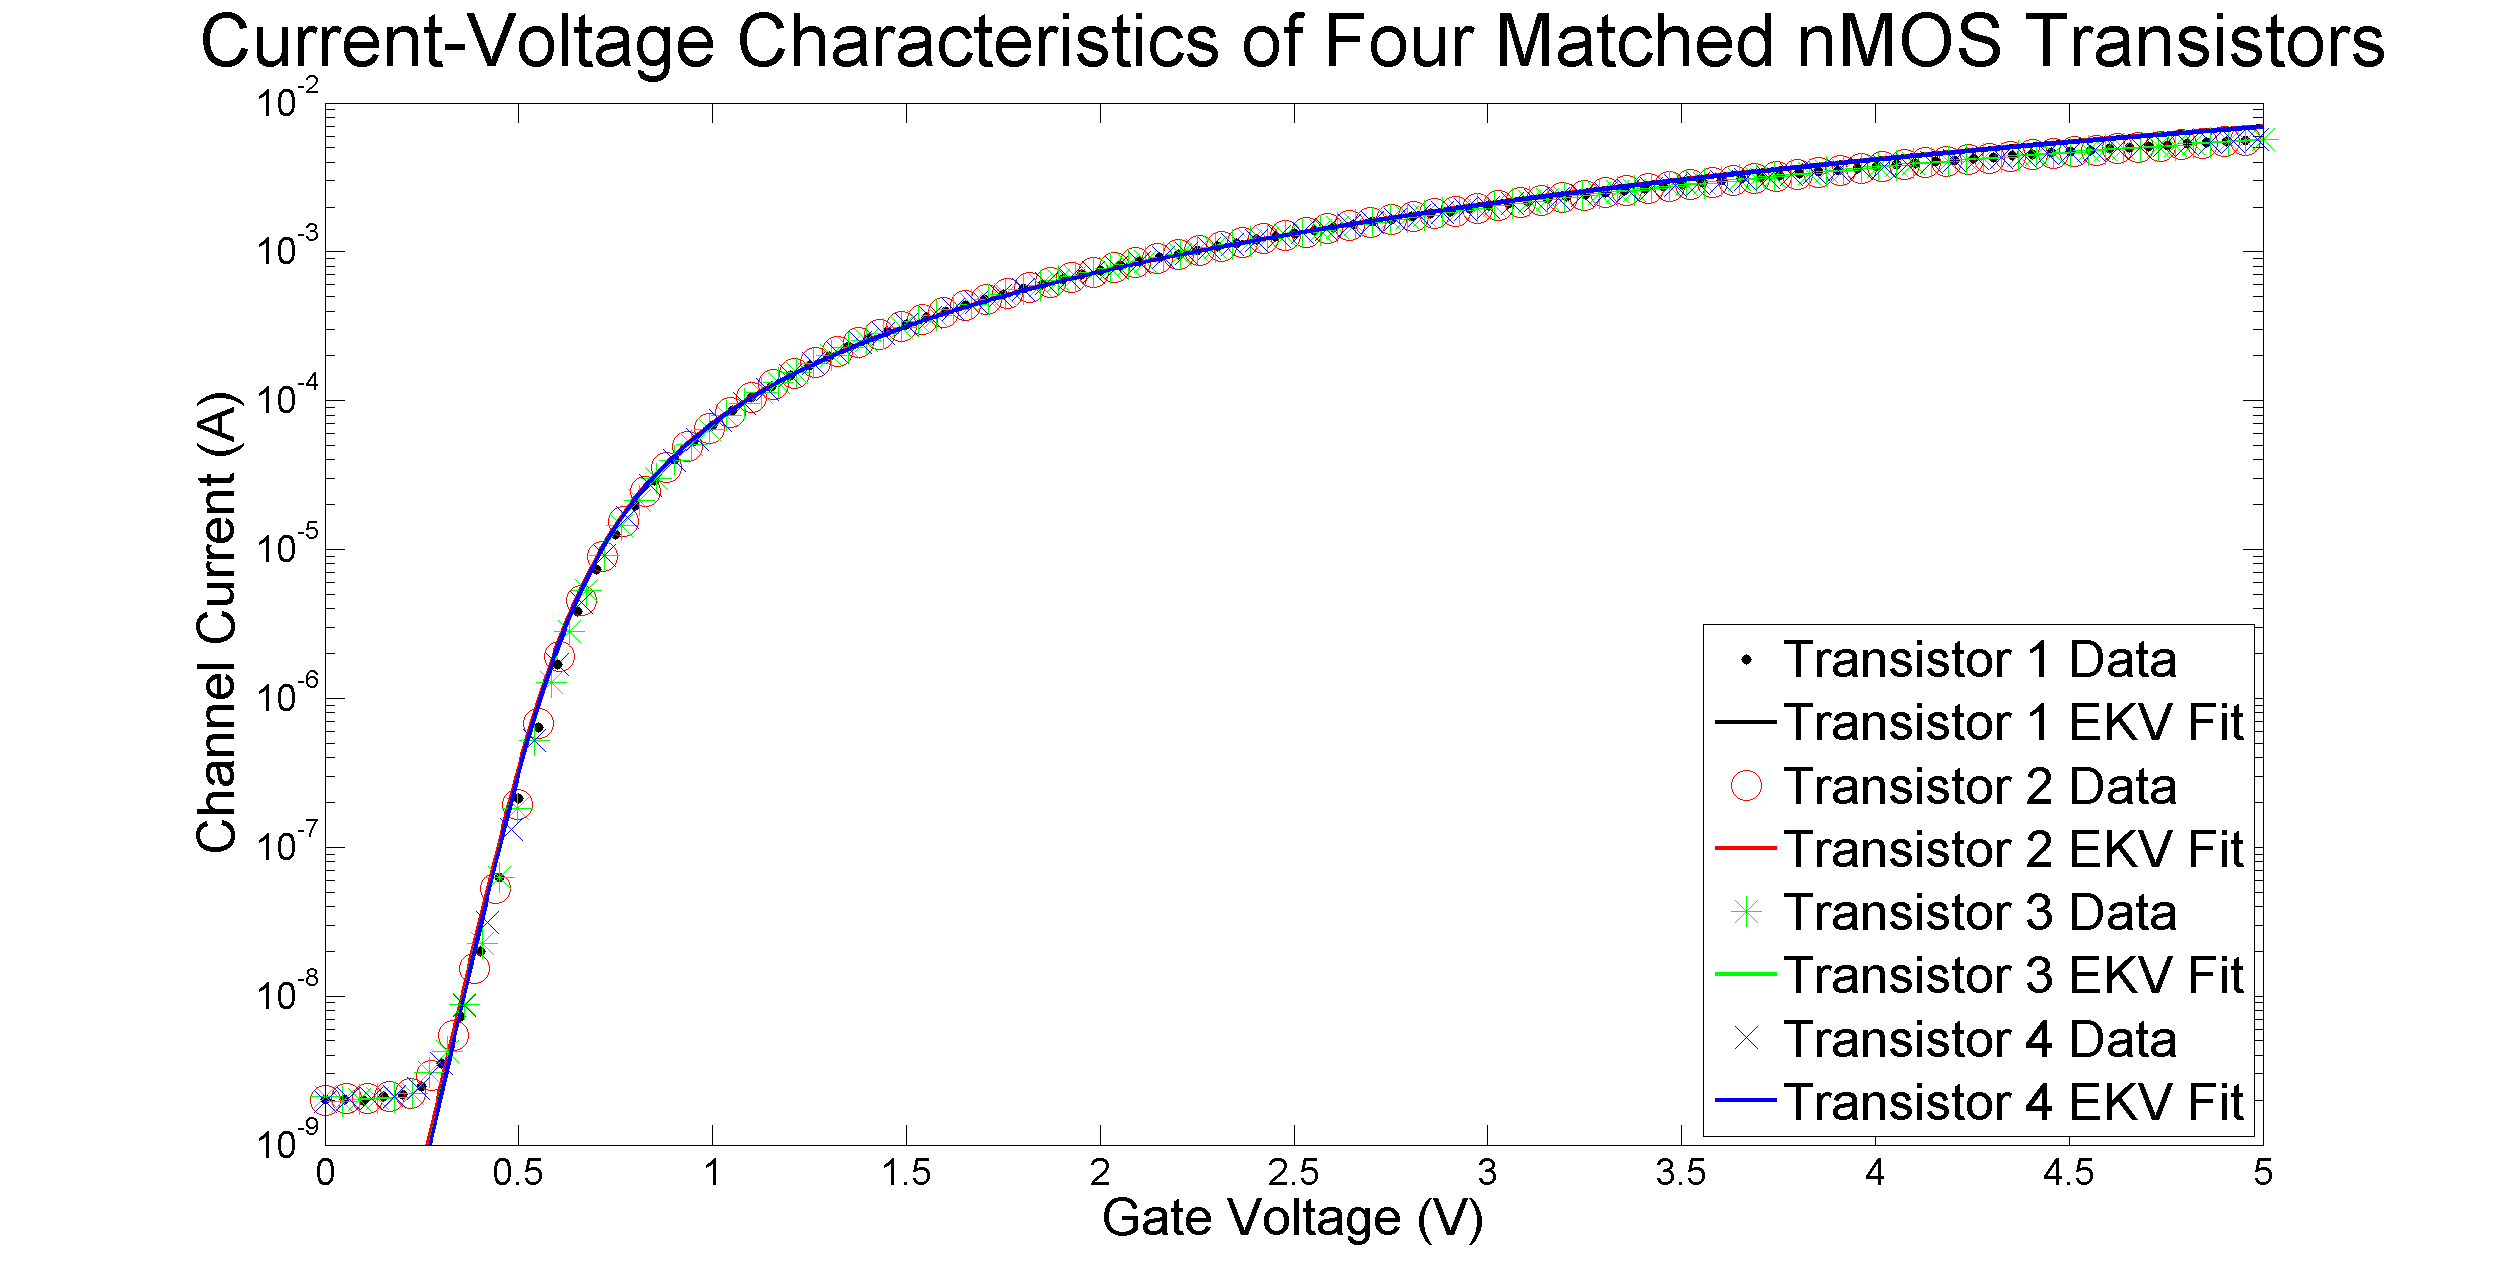
\includegraphics[width=0.65\linewidth]{../Figures/Experiment1Figure1.eps}
\caption{Picture of the ALD1106 QUAD nMOS transistor array which was used in Experiment 1 to analyze the similarities between nMOS transistors. Using a Quad array is ideal as all transistors are manufactured on the same substrate, optimizing their similarity.}
\label{fig:exp1fig1}
\end{figure}
\begin{figure}[H]
\centering
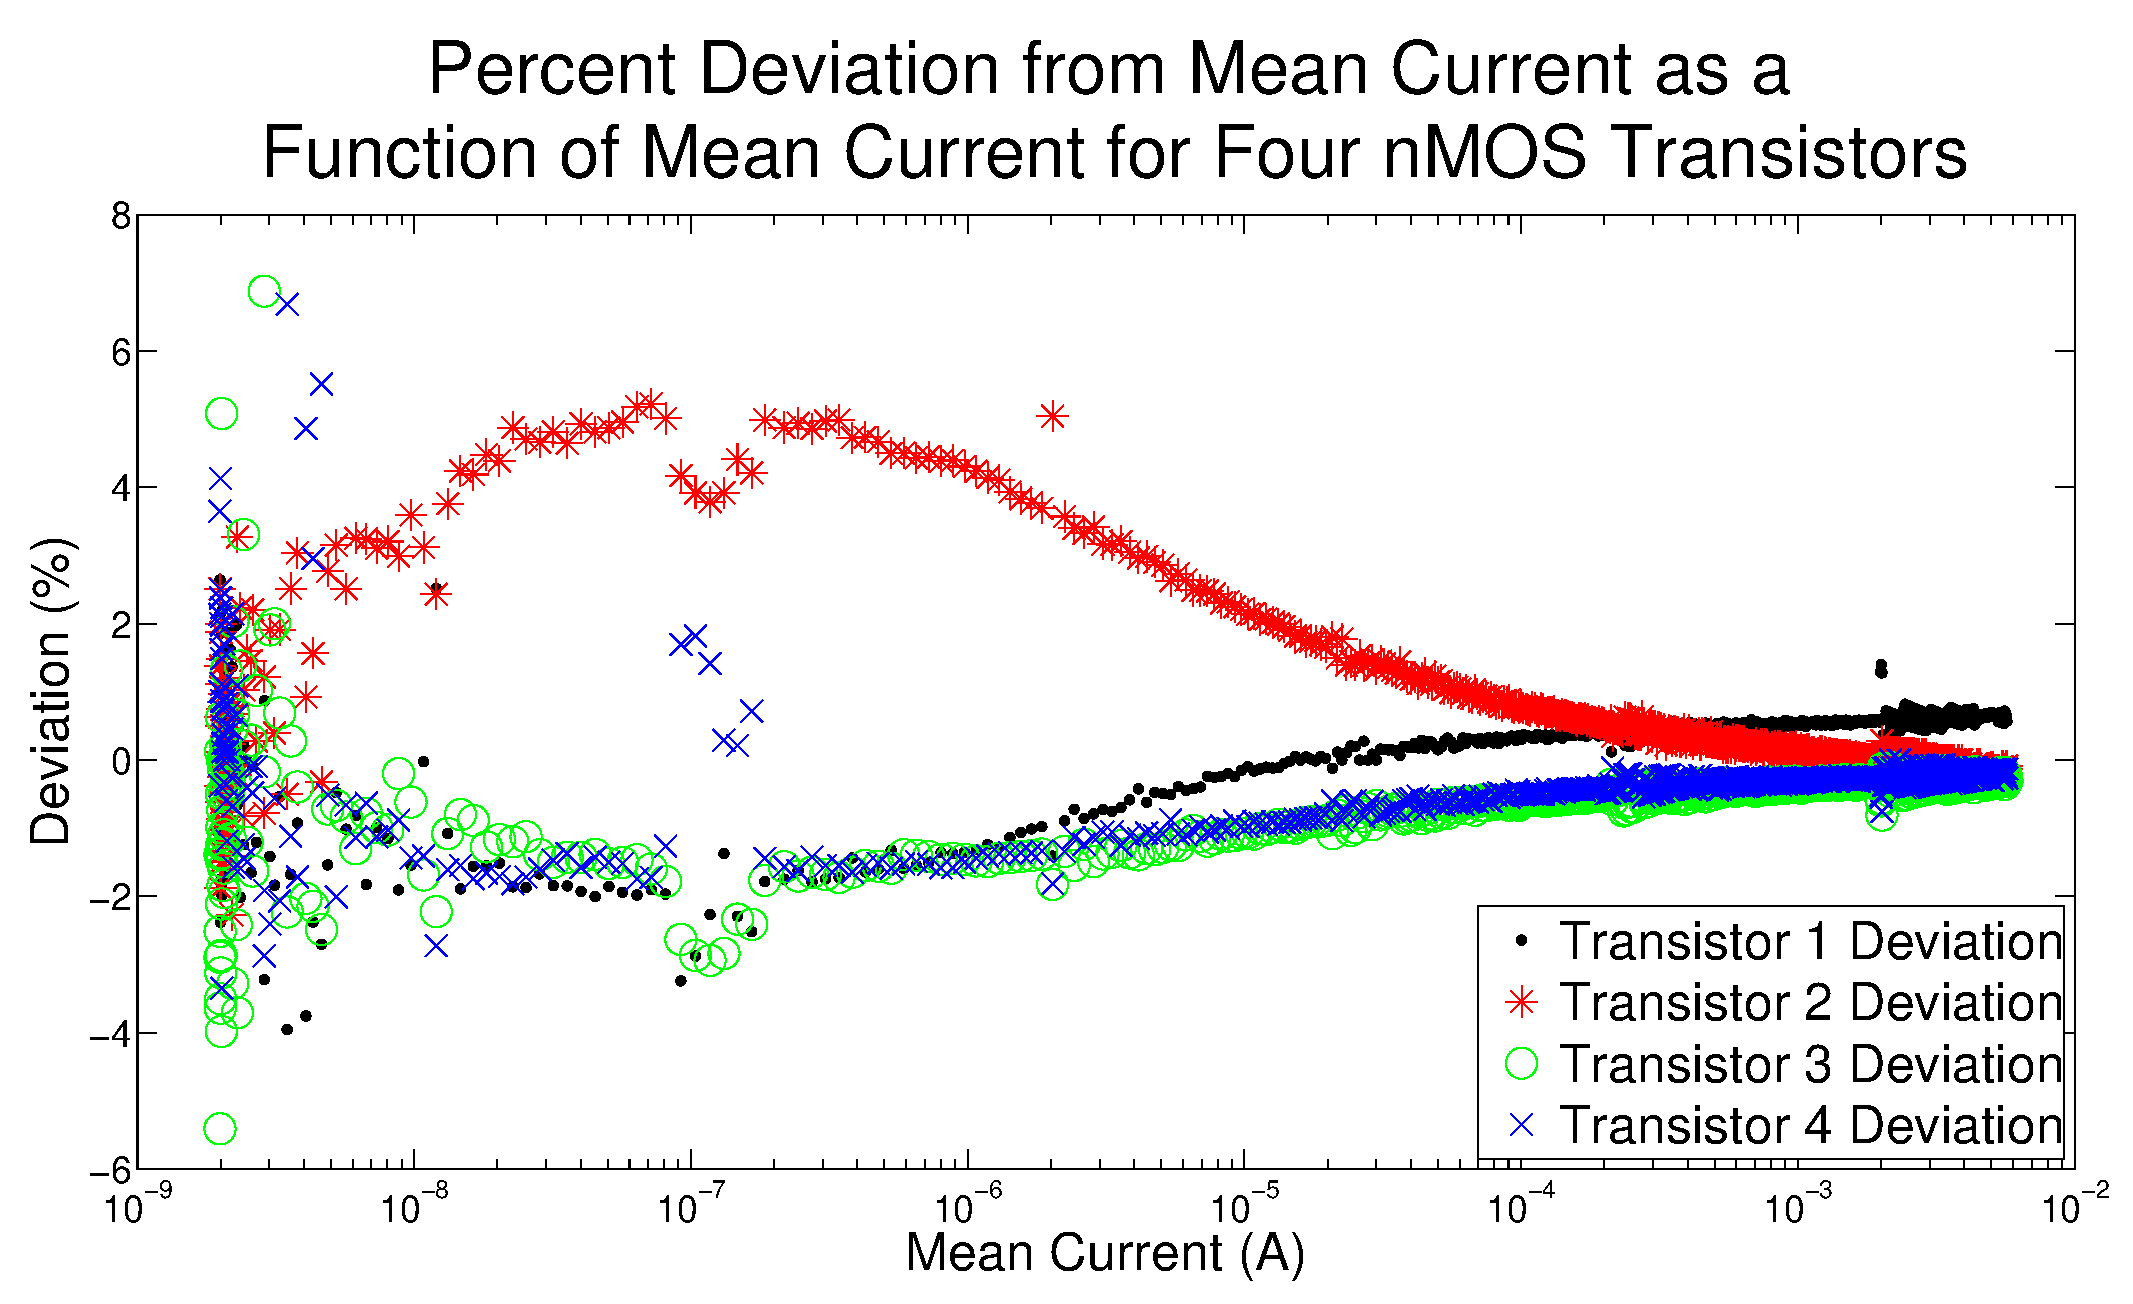
\includegraphics[width=0.65\linewidth]{../Figures/Experiment1Figure2.eps}
\caption{Picture of the ALD1106 QUAD nMOS transistor array which was used in Experiment 1 to analyze the similarities between nMOS transistors. Using a Quad array is ideal as all transistors are manufactured on the same substrate, optimizing their similarity.}
\label{fig:exp1fig2}
\end{figure}